\documentclass{article}

\usepackage{appendix}
\usepackage{todonotes}
\usepackage{wrapfig}
\usepackage{intcalc}
\usepackage{amsthm}
\usepackage{cleveref}

\usepackage{tikz}
\tikzset{%
    simplegraph/.style={every node/.style={draw,circle, inner sep=0pt, minimum size=6mm}},
}
\usetikzlibrary{snakes}
\usetikzlibrary{shapes.geometric}
\usetikzlibrary{positioning, fit, calc}

\usepackage[
	style=alphabetic
]{biblatex}
\addbibresource{bbl.bib}

\newtheorem{theorem}{Theorem}[section]
\newtheorem{corollary}{Corollary}[theorem]
\newtheorem{lemma}[theorem]{Lemma}

\newcommand{\TODO}{\todo[inline]}
\newcommand\Lovasz{Lovász }
\newcommand\T{\mathcal{T}}
\crefname{lemma}{Lemma}{Lemmas}

% Language and typesetting notes:
%
% - Color, not Colour (American English)
% - Node not a Vertex of a graph

\author{Adrian Siwiec}
\date{\today{}}
\begin{document}
\begin{titlepage}
	\begin{center}
        
		\large
		\textbf{Jagiellonian University}\\
		Department of Theoretical Computer Science\\

		\vspace{1.5cm}

		\Large
		\textbf{Adrian Siwiec}

		\vspace*{2cm}

		\textbf{\LARGE Perfect Graph Recognition and Coloring}
		
		\vspace{0.5cm}
		\large
		
		\vfill
		\Large
		Master Thesis

		\vfill
		\Large
		Supervisor: dr inż. Krzysztof Turowski
		
		\vspace{0.8cm}
		
		September 2020
		
\end{center}
\end{titlepage}

\pagebreak

\begin{abstract}
TODO
\end{abstract}

\tableofcontents

\pagebreak

\section{Perfect Graphs}
All graphs in this paper are finite, undirected and have no loops or parallel edges. We denote the chromatic number of graph $G$ by $\chi(G)$ and the cardinality of the largest clique of $G$ by $\omega(G)$. \emph{Coloring} of a graph means assigning every node of a graph a color. A coloring is \emph{valid} iff every two nodes sharing an edge have different colors. An \emph{optimal} coloring (if exists) is a valid coloring using only $\omega(G)$ colors.

Given a graph $G = (V,E)$, sometimes by $V(G)$ and $E(G)$ we will denote a set of nodes and edges of $G$. Given a set $X \subseteq V$ by $G[X]$ we will denote a graph induced on $X$. A graph $G$ is \emph{perfect} iff for all $X \subseteq V(G)$ we have $\chi(G[X]) = \omega(G[X])$.

\paragraph{Editorial notes}
\begin{itemize}
	\item By solid lines we will mark edges, by dashed lines we will mark nonedges, when significant. Sometimes nonedges will not be marked in order not to clutter the image.
	\todo{Where should we put it?}
	\item A node is $X$-complete in $G$ iff it is adjacent to all nodes in $X$.
	\item Given a path $P$, by $P^*$ we will denote its inside.
\end{itemize}

\TODO{Give some examples why are these interesting, some subclasses, and problems that are solvable for perfect graphs, including recognition and coloring}

Given a graph $G$, its \emph{complement} $\overline{G}$ is a graph with the same vertex set and in which two distinct nodes $u, v$ are connected in $\overline{G}$ iff they are not connected in $G$. For example a clique in a graph becomes an independent set in its complement. A perfect graph theorem, first conjured by Berge in 1961 \cite{CB61} and then proven by \Lovasz in 1972 \cite{LL72} states that a graph is perfect iff its complement graph is also perfect. \todo{Should we give some proof of that here? Maybe based on proof in \cite{GC03}}

A \emph{hole} is an induced chordless cycle of length at least 4. An \emph{antihole} is an induced subgraph whose complement is a hole. A \emph{Berge} graph is a graph with no holes or antiholes of odd length.

In 1961 Berge conjured that a graph is perfect iff it is Berge in what has become known as a strong perfect graph conjecture. In 2001 Chudnovsky et al. have proven it and published the proof in an over 150 pages long paper \citetitle{MC06} \cite{MC06}. The following overview of the proof will be based on this paper and on an article withe the same name by Cornuéjols \cite{GC03}.

\subsection{Strong Perfect Graph Theorem}

Odd holes are not perfect, since their chromatic number is 3 and their largest cliques are of size 2. It is easy to see, that an odd antihole of size $n$ has a chromatic number of $\frac{n+1}{2}$ and largest cliques of size $\frac{n-1}{2}$. It is therefore clear, that if a graph is not Berge it is not perfect. To prove that every Berge graph is perfect is the proper part of the strong perfect graph theorem.

\TODO{How long and detailed overview of the proof should we provide?}

\section{Recognizing Berge Graphs}

\TODO{Cite the paper and tell this is only a short overview}

\subsection{Recognition algorithm Overview}

\TODO{Main ideas of the algorithm.}
\TODO{First we check all on $G$, then on $\overline{G}$}

\subsubsection{Simple structures}

\paragraph{Pyramids}

A \emph{path} in $G$ is an induced subgraph that is connected, with at least one node, no cycle and no node of degree larger than 2 (sometimes called chordless path). The \emph{length} of a path or a cycle is the number of edges in it. \todo{Should we move these definitions elsewhere?} A \emph{triangle} in a graph is a set of three pairwise adjacent nodes.

\begin{wrapfigure}[12]{r}{0.35\textwidth}
	\centering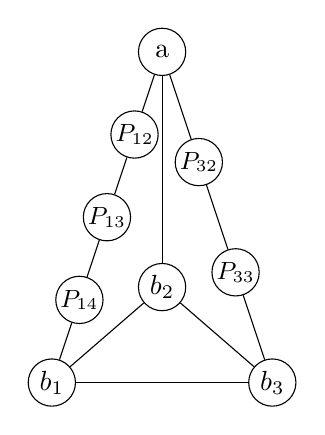
\begin{tikzpicture}[scale=0.7,simplegraph]
	\node(a) at (0,0) {a};
	\node(b1) at (-2,-6) {$b_1$};
	\node(b2) at (0,-4.268) {$b_2$};
	\node(b3) at (2,-6) {$b_3$};

	\node(P12) at (-2/4, -6/4) {\small$P_{12}$};
	\node(P13) at (-4/4, -12/4) {\small$P_{13}$};
	\node(P14) at (-6/4, -18/4) {\small$P_{14}$};

	\node(P32) at (2/3, -6/3) {\small$P_{32}$};
	\node(P33) at (4/3, -12/3) {\small$P_{33}$};

	\draw (b1) to (b3);
	\draw (b1) to (b2);
	\draw (b2) to (b3);

	\draw (a) to (P12);
	\draw (P12) to (P13);
	\draw (P13) to (P14);
	\draw (P14) to (b1);

	\draw (a) to (P32);
	\draw (P32) to (P33);
	\draw (P33) to (b3);

	\draw (a) to (b2);
\end{tikzpicture}
\caption{An example of a pyramid.}
\end{wrapfigure}

A \emph{pyramid} in G is an induced subgraph formed by the union of a triangle $\{b_1,b_2,b_3\}$, three paths $\{P_1, P_2, P_3\}$ and another node $a$, so that:
\begin{itemize}
	\item $\forall_{1\leq i \leq 3}$ $P_i$ is a path between $a$ and $b_i$
	\item $\forall_{1\leq i < j \leq 3}$ $a$ is the only node in both $P_i$ and $P_j$ and $b_ib_j$ is the only edge between $V(P_i)\setminus\{a\}$ and $V(P_j)\setminus\{a\}$.
	\item $a$ is adjacent to at most one of $\{b_1, b_2, b_3\}$.
\end{itemize}

It is easy to see that every graph containing a pyramid contains an odd hole -- at least two of the paths $P_1$, $P_2$, $P_3$ will have the same parity.


\TODO{On recognition of pyramids. Lemma 2.1 from the paper.}

\paragraph{Jewels}


\begin{wrapfigure}[7]{r}{0.35\textwidth}
	\centering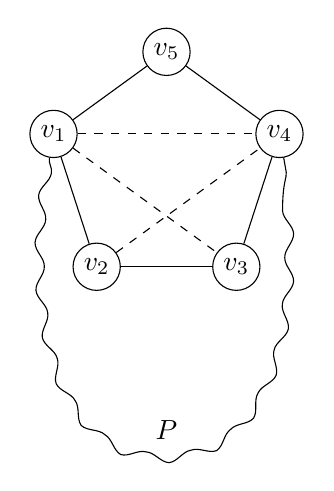
\begin{tikzpicture}[scale=0.7,simplegraph]
	\def\ngon{5}
	\node[regular polygon,regular polygon sides=\ngon,minimum size=3cm, draw=none] (p) {};
	\foreach\x in {1,...,\ngon}{\node[] (p\x) at (p.corner \x){$v_\the\numexpr\intcalcMod{\x+3}{5}+1$};}
	%p1 - v5, p2 - v1 ...
	\draw (p1) to (p2);
	\draw (p2) to (p3);
	\draw (p3) to (p4);
	\draw (p4) to (p5);
	\draw (p1) to (p5);

  \draw[dashed] (p2) to (p5);
  \draw[dashed] (p2) to (p4);
	\draw[dashed] (p3) to (p5);
	
	\tikzset{decoration={snake,amplitude=.6mm,segment length=6mm,
                       post length=0mm,pre length=0mm}}
	\draw[decorate] (p2) to [out=-100, in=180] (0, -5) to [out=0, in=-80] (p5);
	\node[draw=none] at (0, -4.7) {$P$};
\end{tikzpicture}
\caption{An example of a jewel.}
\end{wrapfigure}


Five nodes $v_1, \ldots, v_5$ and a path $P$ is a \emph{jewel} iff:

\begin{itemize}
	\item $v_1, \ldots, v_5$ are distinct nodes.
	\item $v_1v_2, v_2v_3, v_3v_4, v_4v_5, v_5v_1$ are edges.
	\item $v_1v_3, v_2v_4, v_1,v_4$ are nonedges.
	\item $P$ is a path between $v_1$ and $v_4$, such that $v_2, v_3, v_5$ have no neighbors in its inside.
\end{itemize}

Most obvious way to find a jewel would be to enumerate all choices of $v_1, \ldots v_5$, check if a choice is correct and if it is try to find a path $P$ as required. This gives us a time of $O(|V|^7)$. We could speed it up to $O(|V|^6)$ with more careful algorithm, but since whole algorithms takes time $O(|V|^9)$ and our testing showed that time it takes to test for jewels is negligible we used this simple algorithm.

\paragraph{Configurations of type $\T_1$}

A configuration of type $\T_1$ is a hole of length 5. To find it we simply iterate all choices of paths of length of 4, and check if there exists a fifth node to complete the hole. See paragraph \ref{Optimizations} for more implementation details.

\paragraph{Configurations of type $\T_2$}

\begin{wrapfigure}[15]{r}{0.35\textwidth}
	\centering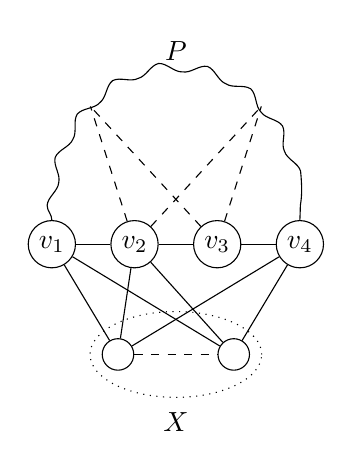
\begin{tikzpicture}[scale=0.7,simplegraph]
		\node(v1) at (0,0) {$v_1$};
		\node(v2) at (1.5,0) {$v_2$};
		\node(v3) at (3,0) {$v_3$};
		\node(v4) at (4.5,0) {$v_4$};

		\draw (v1) to (v2);
		\draw (v2) to (v3);
		\draw (v3) to (v4);

		\tikzset{decoration={snake,amplitude=.6mm,segment length=6mm,
                       post length=0mm,pre length=0mm}}
		\draw[decorate] (v1) to [out=90, in=180] (4.5/2, 3) to [out=0, in=90] (v4);
		\node[draw=none] at (4.5/2, 3.5) {$P$};
		
		\draw[dashed] (v2) to (.7,2.5);
		\draw[dashed] (v3) to (.7,2.5);
		\draw[dashed] (v2) to (3.8,2.5);
		\draw[dashed] (v3) to (3.8,2.5);

		\node[minimum size=4mm](x1) at (1.2, -2){};
		\node[minimum size=4mm](x2) at (3.3, -2){};
		\node[draw,dotted,inner sep=3pt, circle,yscale=.5, fit={(x1) (x2)},label=below:{$X$}] {};

		\draw[dashed] (x1) to (x2);
		\draw(v1) to (x1);
		\draw(v2) to (x1);
		\draw(v4) to (x1);
		\draw(v1) to (x2);
		\draw(v2) to (x2);
		\draw(v4) to (x2);

		% \draw (a) to (b2);
\end{tikzpicture}
\caption{An example of a $\T_2$.}
\end{wrapfigure}

A configuration of type $\T_2$ is a six $(v_1, v_2, v_3, v_4, P, X)$, such that:
\begin{itemize}
	\item $v_1v_2v_3v_4$ is a path in $G$.
	\item $X$ is an anticomponent of the set of all $\{v_1, v_2, v_4\}$-complete nodes.
	\item $P$ is a path in $G\setminus(X \cup \{v_2, v_3\})$ between $v_1$ and $v_4$ and no vertex in $P^*$ is $X$-complete or adjacent to $v_2$ or adjacent to $v_3$.
\end{itemize}

Checking if configuration of type $\T_2$ exists in our graph is straightforward: we enumerate all paths $v_1\ldots v_4$, calculate set of all $\{v_1, v_2, v_4\}$-complete nodes and its anticomponents. Then, for each anticomponent $X$ we check if required path $P$ exists.

To prove that existence of $\T_2$ configuration implies that the graph is not berge, we will need the Roussel-Rubio lemma \cite{RR01} as stated in \cite{MC05} that says:

\begin{lemma}[Roussel-Rubio Lemma]\label{Roussel-Rubio}
	Let $G$ be Berge, $X$ be an anticonnected subset of $V(G)$, $P$ be an odd path $p_1\ldots p_n$ in $G\setminus X$ with length at least 3, such that $p_1$ and $p_n$ are $X$-complete and $p_2, \ldots, p_{n-1}$ are not. Then:
	\begin{itemize}
		\item $P$ is of length at least 5 and there exist nonadjacent $x, y \in X$, such that there are exactly two edges between $x, y$ and $P^*$, namely $xp_2$ and $yp_{n-1}$,
		\item or $P$ is of length 3 and there is an odd antipath joining internal nodes of $P$ with interior in $X$.
	\end{itemize}
\end{lemma}

Now, we shall prove the following:

\begin{lemma}
	If $G$ contains configuration of type $\T_2$ then $G$ is not Berge.
\end{lemma}
\begin{proof}
	Let $(v_1, v_2, v_3, v_4, P, X)$ be a configuration of type $\T_2$. Let us assume that $G$ is not Berge and consider the following:
	\begin{itemize}
		\item If $P$ is even, then $v_1, v_2, v_3, v_4, P, v_1$ is an odd hole,
		\item If $P$ is of length 3. \todo{I merged a couple of proofs from \cite{MC06}, check in the morning if this is correct.} Let us name its nodes $v_1, p_2, p_3, v_4$. It follows from \cref{Roussel-Rubio}, that there exists an odd antipath between $p_2$ and $p_3$ with interior in $X$. We can complete it with $v_2p_2$ and $v_2p_3$ into an odd antihole.
		\item If $P$ is odd with the length of at least 5 \todo{check in the morning}, it follows from \cref{Roussel-Rubio} that we have $x, y \in X$ with only two edges to $P$ being $xp_2$ and $yp_{n-1}$. This gives us an odd hole: $v_2, x, p_2, \ldots, p_{n-1}, y, v_2$.
	\end{itemize} 
\end{proof}

\paragraph{Configurations of type $\T_3$}

A configuration of type $\T_3$ is a sequence $v_1, \ldots, v_6$, $P$, $X$, such that:
\begin{itemize}
	\item $v_1, \ldots v_6$ are distinct nodes.
	\item $v_1v_2$, $v_3v_4$, $v_1v_4$, $v_2v_3$, $v_3v_5$, $v_4v_6$ are edges, and $v_1v_3$, $v_2v_4$, $v_1v_5$, $v_2v_5$, $v_1v_6$, $v_2v_6$, $v_4v_5$ are nonedges.
	\item $X$ is an anticomponent of the set of all $\{v_1, v_2, v_5\}$-complete nodes, and $v_3$, $v_4$ are not $X$-complete.
	\item $P$ is a path of $G \setminus ( X \cup \{v_1, v_2, v_3, v_4\} )$ between $v_5$ and $v_6$ and no node in $P*$ is $X$-complete or adjacent to $v_1$ or adjacent to $v_2$.
	\item If $v_5v_6$ is an edge, then $v_6$ is not $X$-complete.
\end{itemize}

\TODO{image?}

The following algorithm with running time of $O(|V(G)|^6)$ checks whether $G$ contains a configuration of type $T_3$:

For each triple $v_1, v_2, v_5$ of nodes such that $v_1v_2$ is an edge and $v_1v_5, v_2v_5$ are nonedges find the set $Y$ of all $\{v_1, v_2, v_5\}$-complete nodes. For each anticomponent $X$ of $Y$ find the maximal connected subset $F'$ containing $v_5$ such that $v_1, v_2$ have no neighbors in $F'$ and no node of $F'\setminus\{v_5\}$ is $X$-complete. Let $F$ be the union of $F'$ and the set of all $X$-complete nodes that have a neighbor in $F'$ and are nonadjacent to all of $v_1, v_2$ and $v_5$. 

Then, for each choice of $v_4$ that is adjacent to $v_1$ and not to $v_2$ and $v_5$ and has a neighbor in $F$ (call it $v_6$) and a nonneibhbor in $X$, we test whether there is a node $v_3$, adjacent to $v_2, v_4, v_5$ and not to $v_1$, with a nonneibhbor in $X$. If there is such a node $v_3$, find $P$ -- a path from $v_6$ to $v_5$ with interior in $F'$ and return that $v_1, \ldots v_6, P, X$ is a configuration of type $\T_3$. If we exhaust our search and find none, report that graph does not contain it.

To see that the algorithm below has a running time of $O(|V(G)|^6)$, let us note that for each triple $v_1, v_2, v_5$ we examine, of which there are $O(|V(G)|^3)$, there are linear many choices of $X$, each taking $O(|V(G)|^2)$ time to process and generating a linear many choices of $v_4$ which take a linear time to process in turn. This gives us the total running time of $O(|V(G)|^6)$.

We will skip the proof that each graph containing $\T_3$ is not Berge. \todo{Should we include it?} See \cite{MC05} for the proof.

\subsubsection{Amenable holes.}

For a shortest odd hole $C$ in $G$, we will call a node $v \in V(G) \setminus V(C)$ $C$-\emph{major} iff the set of its neighbors in C is not contained in any 3-node path of $C$. An odd hole $C$ will be called \emph{clean} if no vertex is $C$-major.

A hole $C$ of $G$ is \emph{amenable} iff C is a shortest odd hole in $G$ of length at least 7, and for every anticonnected set $X$ of $C$-major nodes, there is an $X$-complete edge in $C$ (an edge is $X$-complete iff both its ends are $X$-complete).

The rest of the algorithm rests upon the following theorem:

\begin{theorem}
	Let $G$ be a graph, such that $G$ and $\overline{G}$ contain no Pyramid, no Jewel and no configuration of types $\T_1, \T_2$ or $\T_3$. Then every shortest hole in $G$ is amenable.
	\TODO{Any ideas on what else to say here? List all 9 steps?}
\end{theorem}

For a shortest odd hole $C$ in $G$, a subset $X$ of $V(G)$ is a \emph{near-cleaner for $C$} iff $X$ contains all $C$-major nodes and $X \cap V(C)$ is a subset of node set of some 3-node path of $C$.

Finding and Using Half-Cleaners.\\

Overview of proof of why algorithm using Half-Cleaners is correct.\\

\subsection{Implementation}

Anything interesting about algo/data structure?\\

\subsubsection{Optimizations}\label{Optimizations}
Bottlenecks in performance (next path, are vectors distinct etc).\\
\TODO{In our graph preprocessing we have a pointer to next edge in order to speed up generating next path.}
\TODO{We used callgrind to get idea of methods crucial for time.}
\TODO{In general enumerating all paths is crucial. As is checking if vector has distinct values.}
\TODO{Jewels -- we iterate all possibly chordal paths and check if they are ok - much faster}
\TODO{$\T_1$ -- we iterate all paths of length 4 and check if there exists a fifth node to complete the hole - much faster than iterating nodes.}

Validity tests - unit tests, tests of bigger parts, testing vs known answer and vs naive.

\subsection{Parallelism with CUDA (?)}

TODO

\subsection{Experiments}

Naive algorithm - brief description, bottlenecks optimizations (makes huge difference).\\

Description of tests used.\\

Results and Corollary - almost usable algorithm.



\section{Coloring Berge Graphs}

\subsection{Ellipsoid method}

Description.\\

Implementation.\\

Experiments and results.\\

\subsection{Combinatorial Method}

Cite the paper.\\

On its complexity - point to appendix for pseudo-code.

\appendix
\appendixpage
\addappheadtotoc

\section{Perfect Graph Coloring algorithm}
TODO


% \bibliographystyle{alpha}
\printbibliography

\end{document}